
\begin{figure}[H]
\noindent\centering{
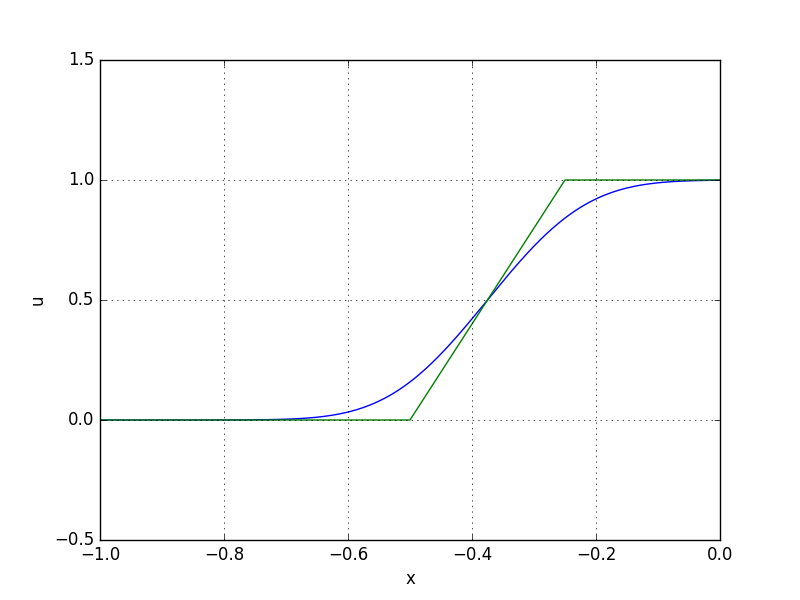
\includegraphics[width=95mm]{img/1-1.png} 
  \caption{Явный линейный}}
\end{figure}

\begin{figure}[H]
\noindent\centering{
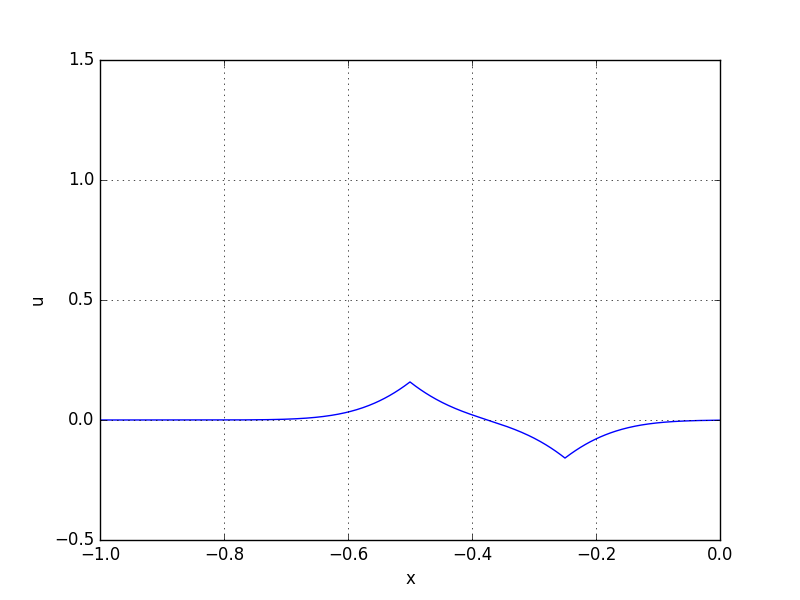
\includegraphics[width=95mm]{img/1-1d.png} 
  \caption{Явный линейный (ошибка)}}
\end{figure}

\begin{figure}[H]
\noindent\centering{
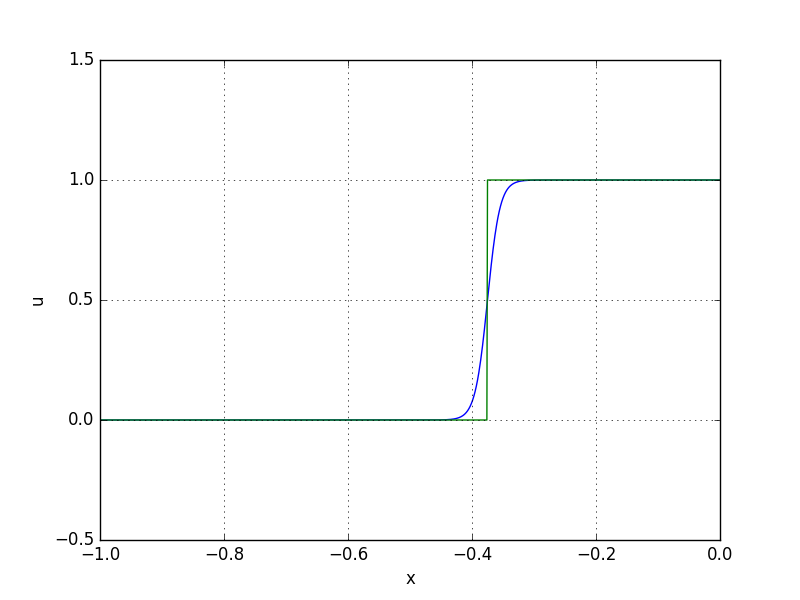
\includegraphics[width=95mm]{img/2-1.png} 
  \caption{Явный нелинейный}}
\end{figure}

\begin{figure}[H]
\noindent\centering{
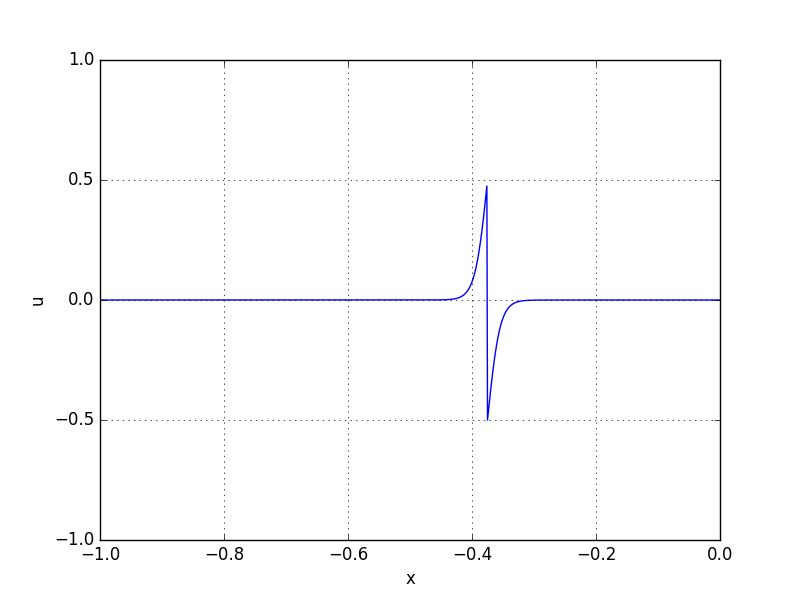
\includegraphics[width=95mm]{img/2-1d.png} 
  \caption{Явный нелинейный (ошибка)}}
\end{figure}

\begin{figure}[H]
\noindent\centering{
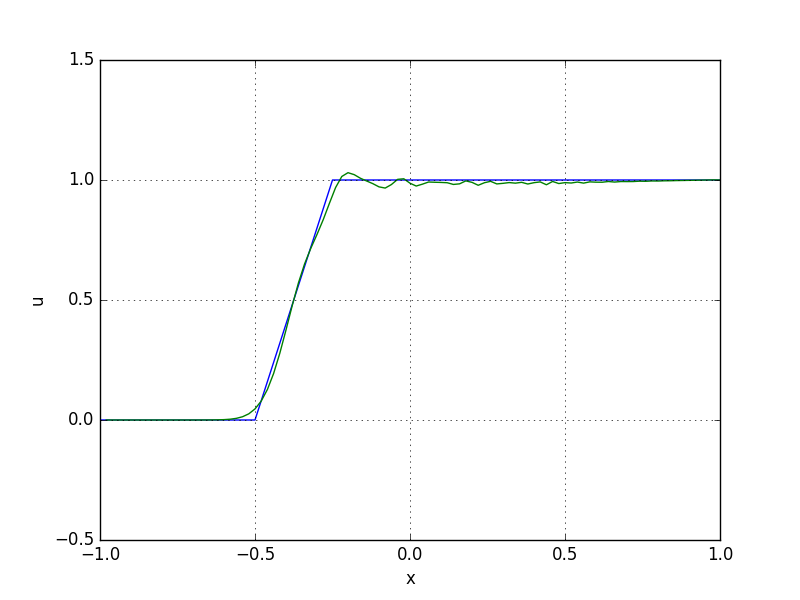
\includegraphics[width=95mm]{img/w=10.png} 
  \caption{Невный линейный $\omega = 1.0$}}
\end{figure}

\begin{figure}[H]
\noindent\centering{
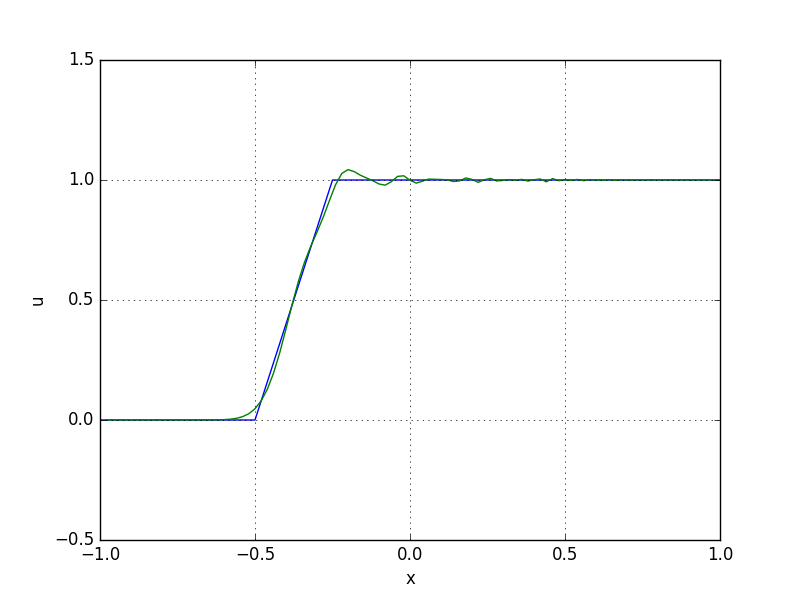
\includegraphics[width=95mm]{img/w=01.png} 
  \caption{Невный линейный $\omega = 0.1$}}
\end{figure}